%%%%%%%%%%%%%%%%%%%%%%%%%%%%%%%%%%%%%%%%%%%%%%%%%%%%%%%%%%%%%%%%%%%%%%%%%%%%%
%% MS Draft Journal of Ecology Special Issue, Dispersal - SUPPL MATERIAL
%% Pedro - 07 June 2016
%----------------------------------------------------------------------------
%%%%%%%%%%%%%%%%%%%%%%%%%%%%%%%%%%%%%%%%%%%%%%%%%%%%%%%%%%%%%%%%%%%%% Headers
\documentclass[a4paper, 12pt]{article}
\usepackage{graphicx}
\usepackage[utf8]{inputenc}
\usepackage[a4paper]{geometry}
\usepackage{hyperref}
\pagestyle{plain}
\usepackage{amsmath,amssymb}
\usepackage{geometry}
\usepackage{lscape}
\usepackage{setspace}
\usepackage{verbatim}
\usepackage{graphicx}
\usepackage{epstopdf}
\usepackage{booktabs}
\usepackage{natbib}
\usepackage{longtable}
\usepackage{rotating}                                                                                     
\newcommand{\tab}{\hspace{5mm}}
\usepackage{tabularx} 
\usepackage[margin=10pt,font=small,labelfont=bf]{caption}
\usepackage[left]{lineno}
\usepackage{caption}
\DeclareGraphicsRule{.tif}{png}{.png}{`convert #1 `basename #1 .tif`.png}
\usepackage{fancyhdr} % This should be set AFTER setting up the page geometry
\pagestyle{empty}     % options: empty , plain , fancy
\renewcommand{\headrulewidth}{0pt} % customise the layout...
\lhead{{\tiny Jordano - What is long-distance dispersal?}}\chead{}\rhead{}
\lfoot{}\cfoot{\thepage}\rfoot{}
\usepackage{parskip}
\linespread{1.25}
%%%%%%%%%%%%%%%%%%%%%%%%%%%%%%%%%%%%%%%%%%%%%%%%%%%%%%%%%%%%%%%%%% Title page
\begin{document}


\title{Manuscript Draft\\
\vspace{2cm}
What is long-distance dispersal? And a taxonomy of dispersal events \\
\textbf{Supplementary Material}}

\author{Pedro Jordano$^{\dag}$}

\date{Sevilla, \today}
\maketitle


\begin{spacing}{1.0}
$^{\dag}$ {\small Integrative Ecology Group, Estaci\'on Biol\'ogica de 
Do\~nana, CSIC, Avda. Americo Vespucio, s/n, Isla de La Cartuja
E-41092 Sevilla, Spain.}\\


{\small \textit{Corresponding author:} Pedro Jordano. Integrative Ecology Group, Estaci\'on Biol\'ogica de Do\~nana, CSIC, Avda. americo Vespucio, s/n, E-41092 Sevilla, Spain. Email address: jordano@ebd.csic.es}\\

\textbf{Key words}: ***\\

{\small \textbf{Manuscript information: }** Words; ** Chars; ** Pages, * Figures; * Tables.}
\end{spacing}

\maketitle
\newpage

%%%%%%%%%%%%%%%%%%%%%%%%%%%%%%%%%%%%%%%%%%%%%%%%%%%%%% Supplementary Material
%------------------------------------------------------------------- Table S1
\begin{landscape}
\begin{table}
  \caption{Summary of neighborhood area sizes and estimated neighborhood radius for tree species with different combinations of dispersal modes. Data from Nason et al and present study. }
    \begin{tabular}{lllccc}
     Species                & Pollinator  & Seed disperser & Density ($ha^{-1}$) & Breeding unit ($km^2$) & Radius (km) \\
    \textit{Ficus dugandii}          & Fig wasp    & Vertebrates    & 0.004          & 631.7               & 14.2        \\
    \textit{Ficus obtusifolia}       & Fig wasp    & Vertebrates    & 0.072          & 105.9               & 5.8         \\
    \textit{Prunus mahaleb}          & Bees, flies & Vertebrates    & 0.003          & 0.87                & 0.042       \\
    \textit{Frangula alnus}          & Bees, flies & Vertebrates    & 0.0004         & 0.45                & 0.013       \\
    \textit{Astrocaryum mexicanum}   & Beetle      & Vertebrates    & 1364.0         & 0.011               & 0.06        \\
    \textit{Calophyllum longifolium} & Bees        & Vertebrates    & 0.28           & 1.241               & 0.629       \\
    \textit{Platypodium elegans}     & Bees        & Wind           & 0.78           & 0.866               & 0.525       \\
    \textit{Cedrus atlantica}        & Wind        & Wind           & 61.7           & 0.151               & 0.22        \\
   \textit{Fraxinus americana}      & Wind        & Wind           & 24.7           & 0.008               & 0.05        \\
    \textit{Pseudotsuga menziesii}   & Wind        & Wind           & 25.0           & 0.078               & 0.158       \\
    \end{tabular}
\end{table}
\end{landscape}
\newpage 

%------------------------------------------------------------------ Figure S1
\begin{figure}[htbp]
\centerline{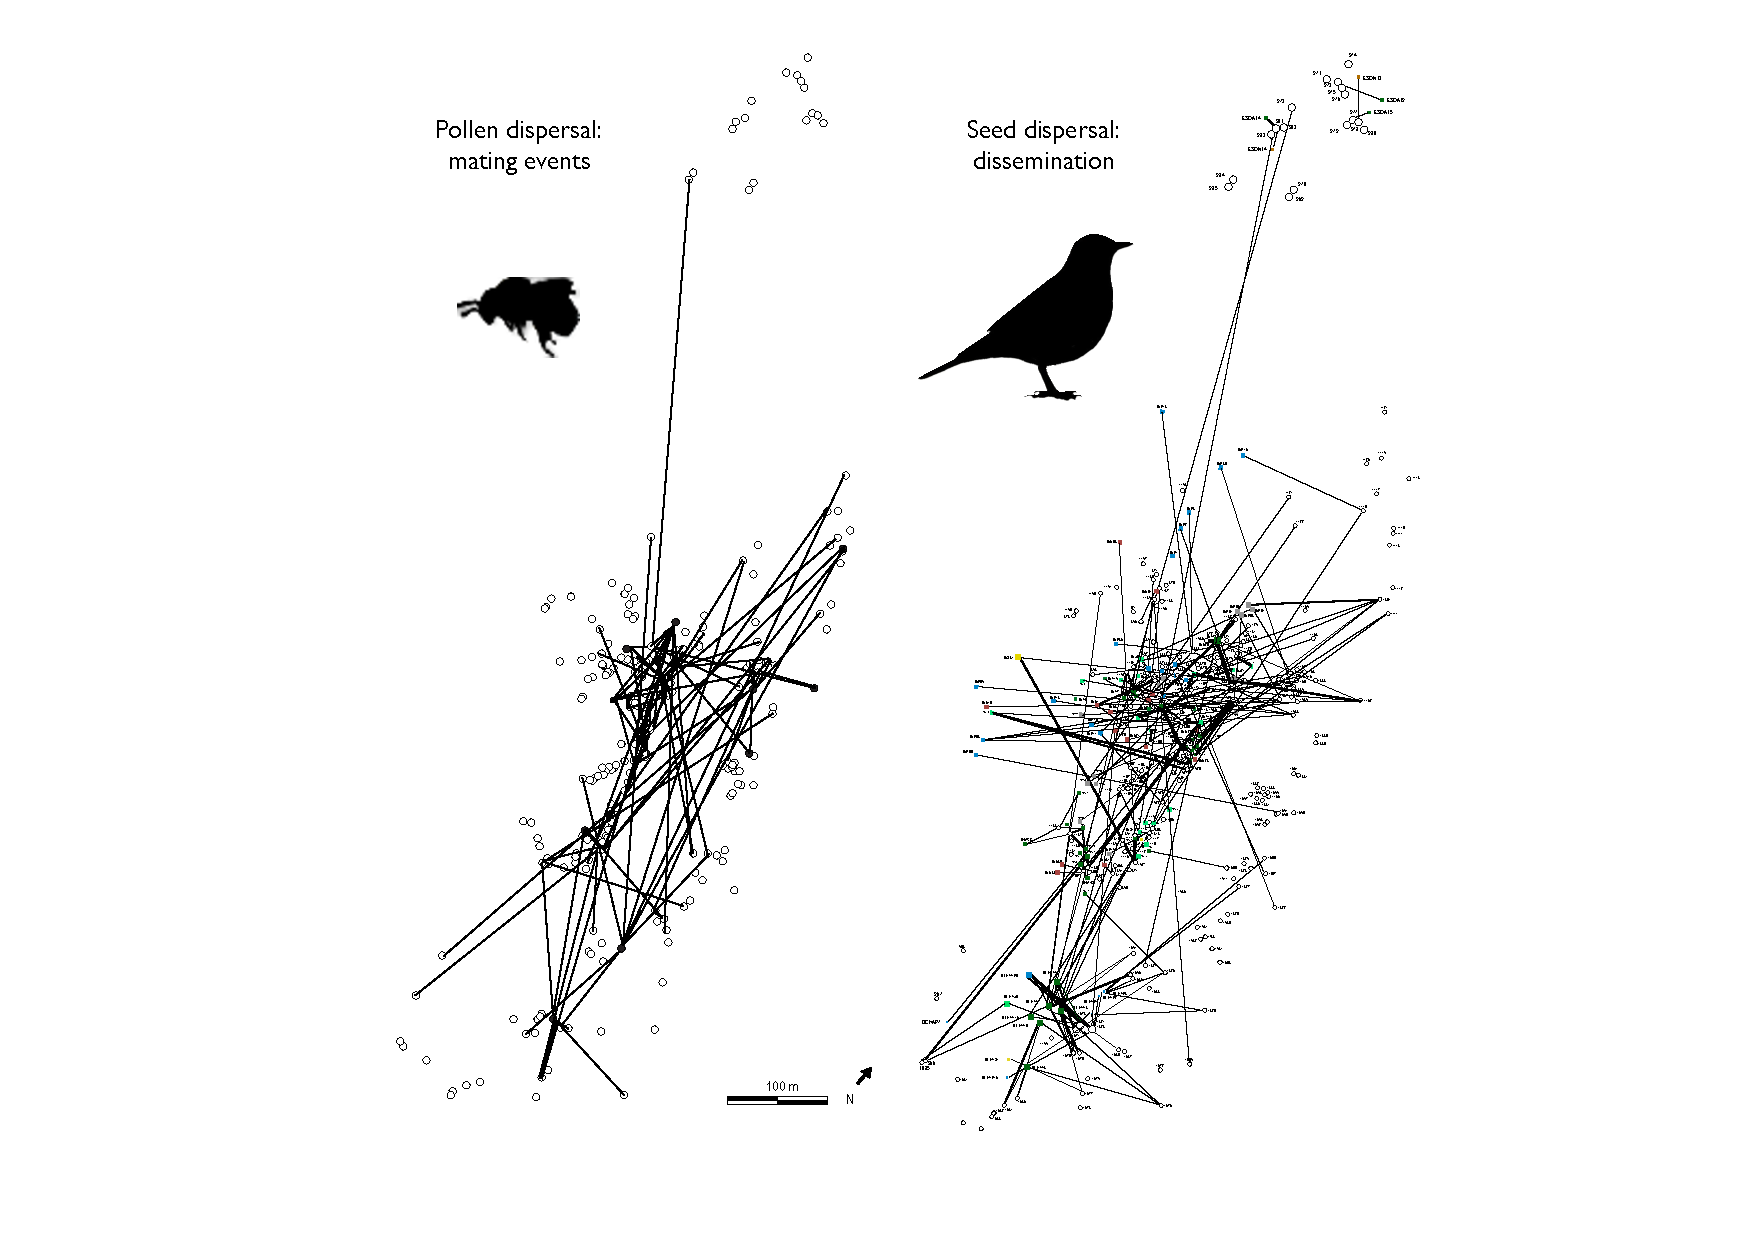
\includegraphics[height=21cm]{FigS1.pdf}}
%
\caption{Dispersal events for pollen (left) and seeds (right) traced for \textit{Prunus mahaleb} trees (white dots). All the adult, reproductive, trees in the population are mapped. Lines indicate mating events of pollen dispersal among trees (left) or seed dissemination events from source fruiting trees to seed traps (squares; right). Line thickness is proportional to the number of events recorded.}
\end{figure}

\newpage 

%------------------------------------------------------------------ Figure S2
\begin{figure}[htbp]
\centerline{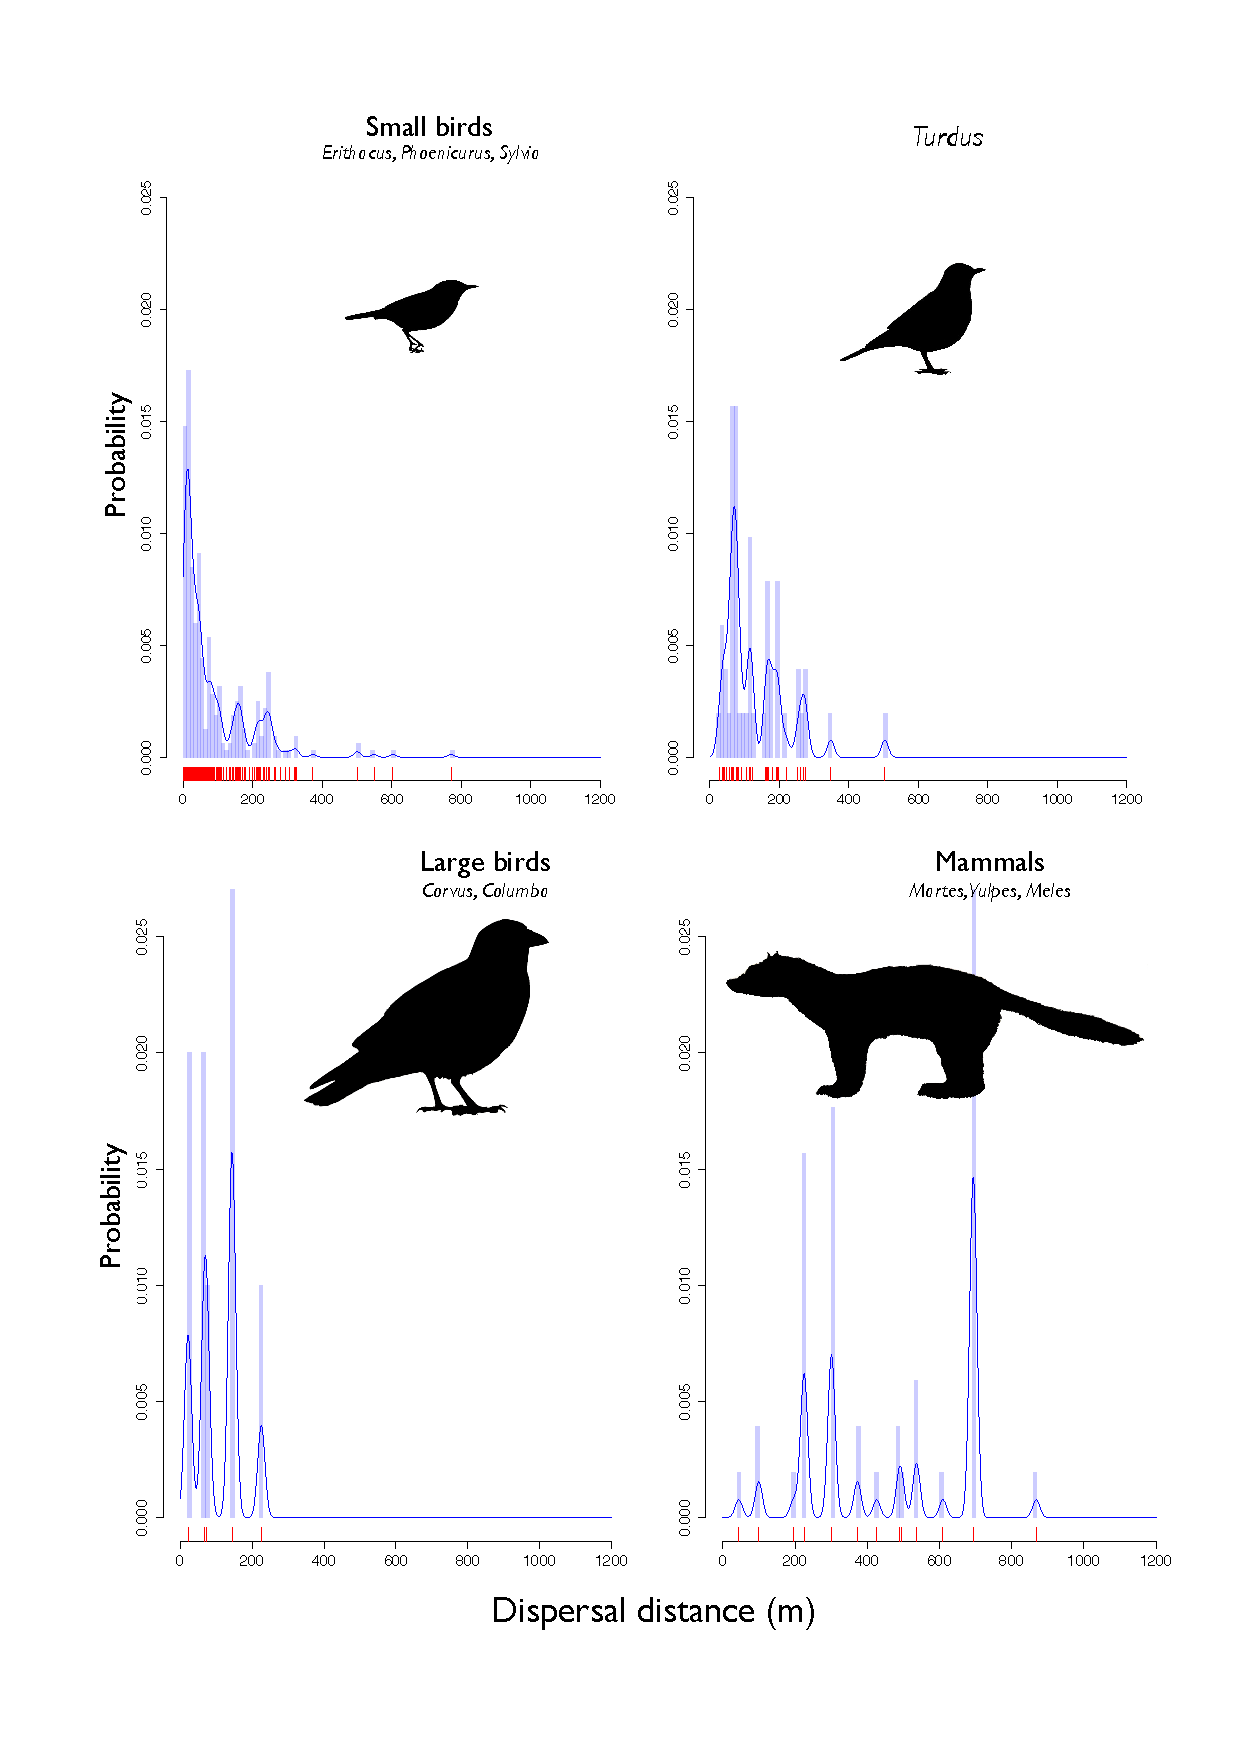
\includegraphics[height=22cm]{FigS2.pdf}}
%
\caption{Differential contributions of functional groups of frugivores to the short- ($SDD_{loc}$) and long-distance ($LDD_{loc}$) local seed dispersal events for \textit{Prunus mahaleb}.}
\end{figure}

\newpage 

%%%%%%%%%%%%%%%%%%%%%%%%%%%%%%%%%%%%%%%%%%%%%%%%%%%%%%%%%%%%%%%%%%%%%%%%%%%%%
	
\end{document}
